\section{Experiments}
\label{expts}

\def\grad{\nabla}
\def\wtilde{\tilde{w}}
\def\Cone{{\cal{C}}^1}
\def\kappap{\kappa^\prime}
\def\Lhat{\hat{L}}
\def\fhat{\hat{f}}
\def\what{\hat{w}}
\def\dhat{\hat{d}}
\def\mysgn{\operatorname{sgn}}


%\def\kdd{{\it{kdd2010}}}
%\def\webspam{{\it{webspam}}}
%\def\url{{\it{url }}}
%\def\sqm{{\it{SQM }}}
%\def\hybrid{{\it{HYBRID }}}
%\def\oursvrg{{\it{FS-k }}}
%\def\ourtron{{\it{FT-k }}}


In this section, we demonstrate the effectiveness of our method on large dimensional data sets. We first discuss our experimental setup. We then show results
to validate the theory proposed in the paper. Finally, we compare our approach with existing distributed machine learning algorithms and clearly demonstrate scenarios under which our method performs better.

\subsection{Experimental Setup}
We run our experiments on a Hadoop cluster. Since iterations in traditional MapReduce are slower (because of job setup and disk access costs), as in Agarwal et al.~\yrcite{agarwal2011}, we build an AllReduce binary tree between the mappers\footnote{Note that we do not use the pipelined version and hence we incur an extra multiplicative $logP$ cost in communication.}. The communication bandwidth is $1 Gbps$ (gigabits per sec).  For functional approximation we use (\ref{riskapp}) and (\ref{linapp}). We use the Area under Precision-Recall Curve (AUPRC) and difference to the optimal function value as the evaluation criteria.\vspace{0.1in} \\

\begin{table}[ht]
\caption{Datasets} % title of Table
\centering % used for centering table
\begin{tabular}{c c c c c c c} % centered columns (4 columns)
\hline\hline %inserts double horizontal lines
Dataset & Examples & Features & Non-zeros\\ %[0.5ex] % inserts table
%heading
\hline 
{\it{kdd2010}} & $8.41M$ & $20.21M$ & 0.31B\\
{\it{url }} & $1.91M$ &  $3.23M$ &  0.22B\\
\hline 
\end{tabular}
\label{tab:params}
\end{table}

{\bf{Data Sets. }}We consider two well known large dimensional datasets: {\it{kdd2010}}  and {\it{url}}. Table~\ref{tab:params} shows the number of examples, features and nonzero feature values. We use these datasets mainly to illustrate the validity of theory, and its utility to distributed machine learning.\vspace{0.1in} \\
%illustration purpose only
{\bf{Methods for Comparison. }}We use the {\it{squared-hinge}} loss function with {\it{l2}}-regularization for all the experiments. We compare the following methods.

%\begin{itemize}
%\item {\bf{{\it{SQM}}: }}
\noindent{\bf{{\it{SQM: }}}}We use the Trust Region Newton method (TRON) proposed in Lin et al.~\yrcite{lin2008} and, do the gradient and Hessian computations in a parallel manner. We initialize the weight vector to zero and set all the parameters (except regularizer $\lambda$) to the values recommended in Lin et al.~\yrcite{lin2008}.
%\item {\bf{{\it{HYBRID}: }}

\noindent{\bf{{\it{HYBRID: }}}}We find a local weight vector per node by minimizing the local objective function (based only on the examples in that node) using one epoch of SGD~\cite{bottou2010}. (The optimal step size is chosen by running SGD on a subset of data.) We then average the weights from all the nodes and use the averaged weight vector to warm start {\it{SQM}}. Note that this method is same as that proposed in Agarwal et al.~\yrcite{agarwal2011} (except that they use the L-BFGS method instead of TRON).

\noindent{\bf{{\it{FS-k: }}}}Our algorithm with the SVRG method~\cite{johnson2013} used for solving the local optimization in every iteration. As suggested in~\cite{johnson2013}, we recalculate the batch gradient after every $5$ epochs (referred as outer iteration in the local optimization context). We run $k$ outer iterations of SVRG and show results for $k=8$ and $16$.

\noindent {\bf{{\it{FT-k: }}}}Our algorithm with TRON~\cite{lin2008} used for solving the local optimization. We stop the inner optimization after doing $k$ Hessian-vector multiplications. The results are shown for $k=50$ and $100$ for {\it{kdd2010}} and $k=25$ and $50$ for {\it{url}}.
%\end{itemize}

%In our algorithms we restricted the number of line search steps to $10$. Note that both TRON and SVRG are state of the art solvers and meet our condition of early stopping required in Theorem 4.

%choice of number of inner iterations is dependent on number of nodes
%say that do not use outer iterations
%ours is good global cnvergence and slow local movement vice versa for them
%wrt no. of nodes vs. ours
%tron vs. svrg

\begin{figure}[t]
\centering
\subfigure[{\it{kdd2010}} - 25 nodes]{
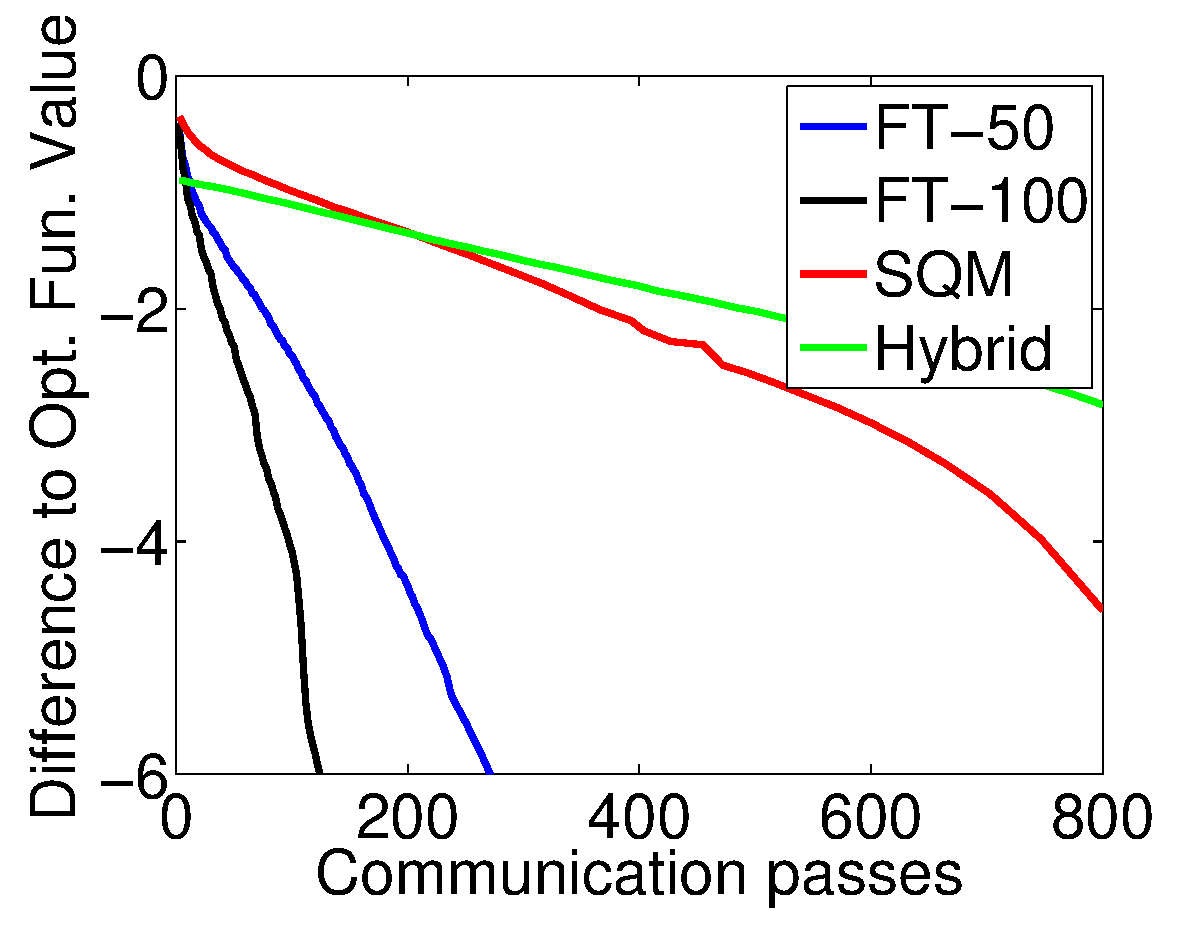
\includegraphics[width=0.46\linewidth]{figures/kddtron_25nodes_outeriters.eps}
}
\subfigure[{\it{kdd2010}} - 100 nodes]{
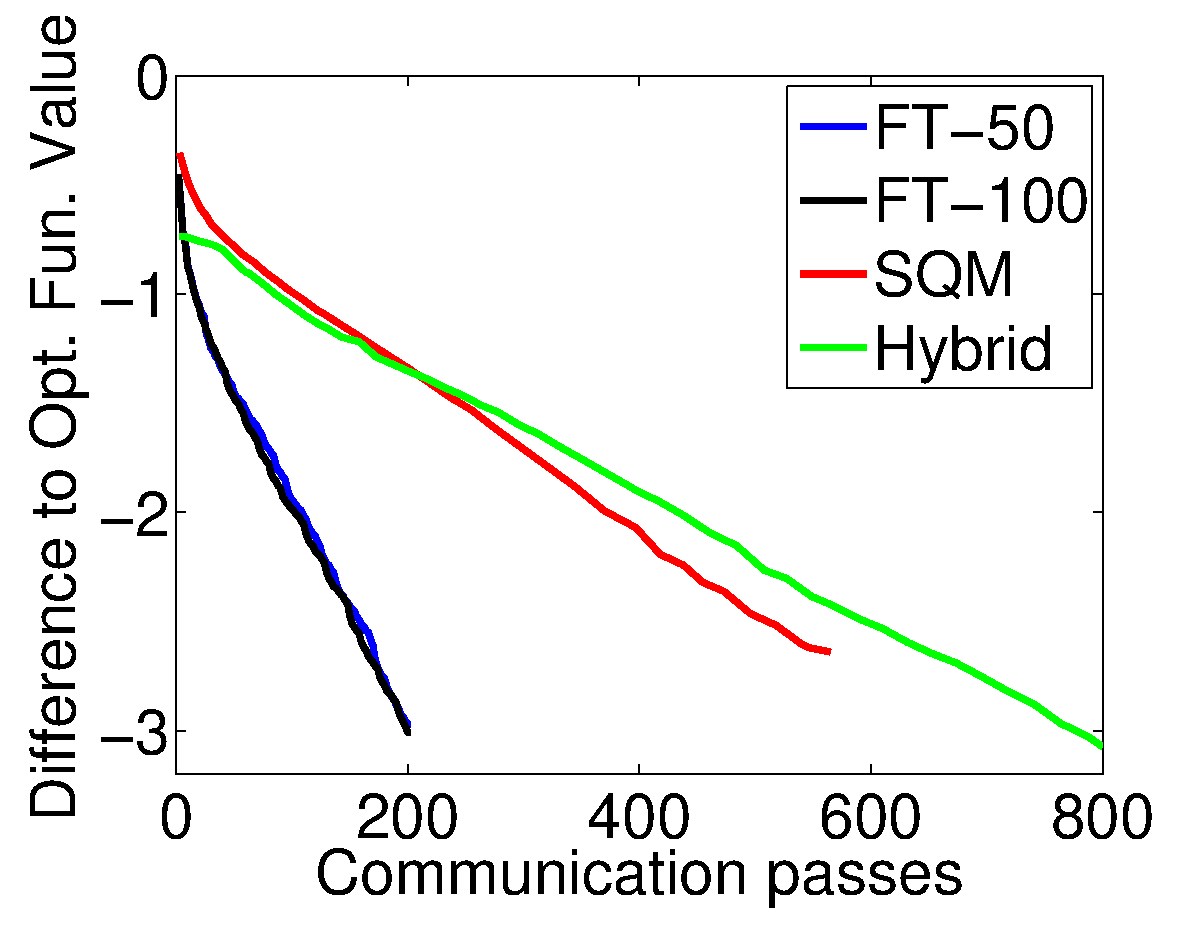
\includegraphics[width=0.46\linewidth]{figures/kddtron_100nodes_outeriters.eps}
}
\subfigure[{\it{url}} - 6 nodes]{
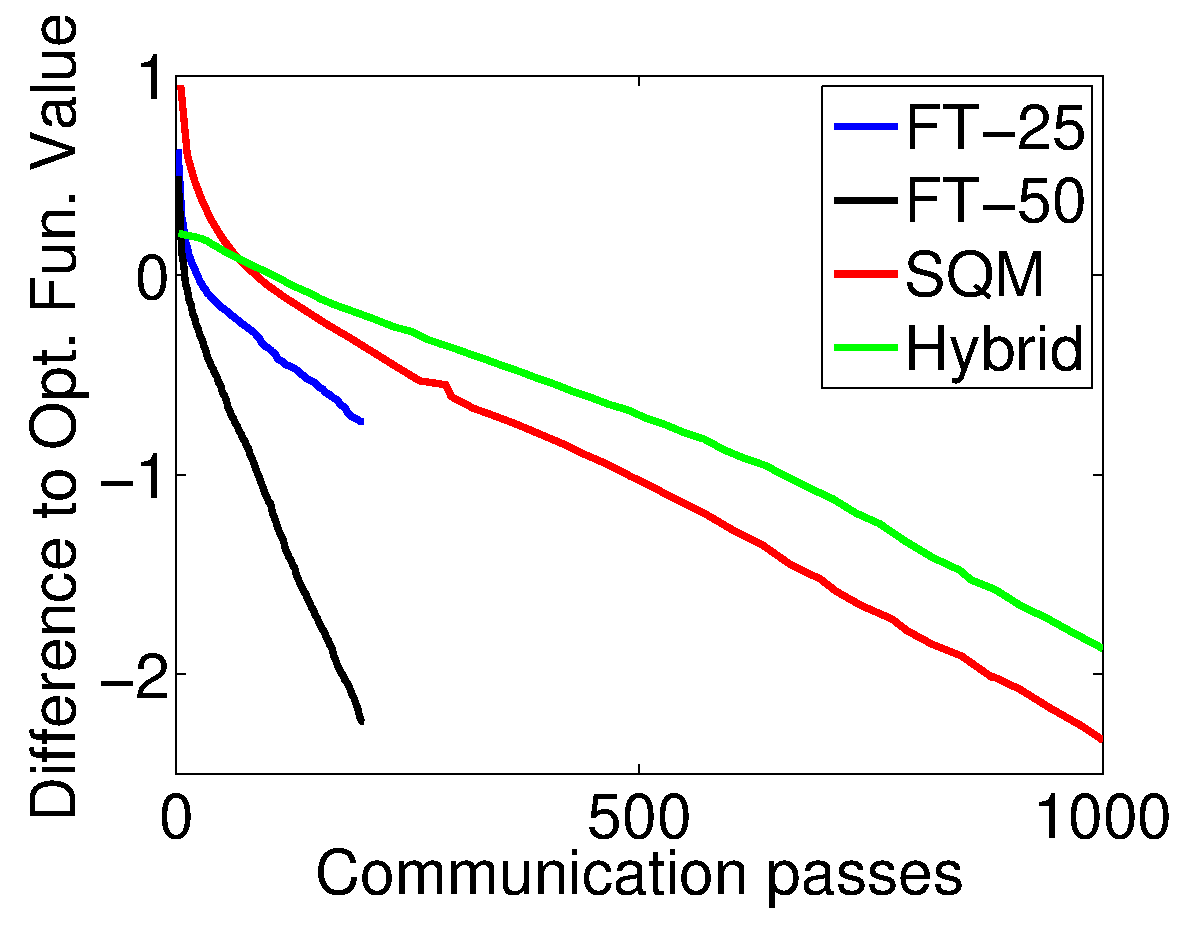
\includegraphics[width=0.46\linewidth]{figures/urltron_6nodes_outeriters.eps}
}
\subfigure[{\it{url}} - 100 nodes]{
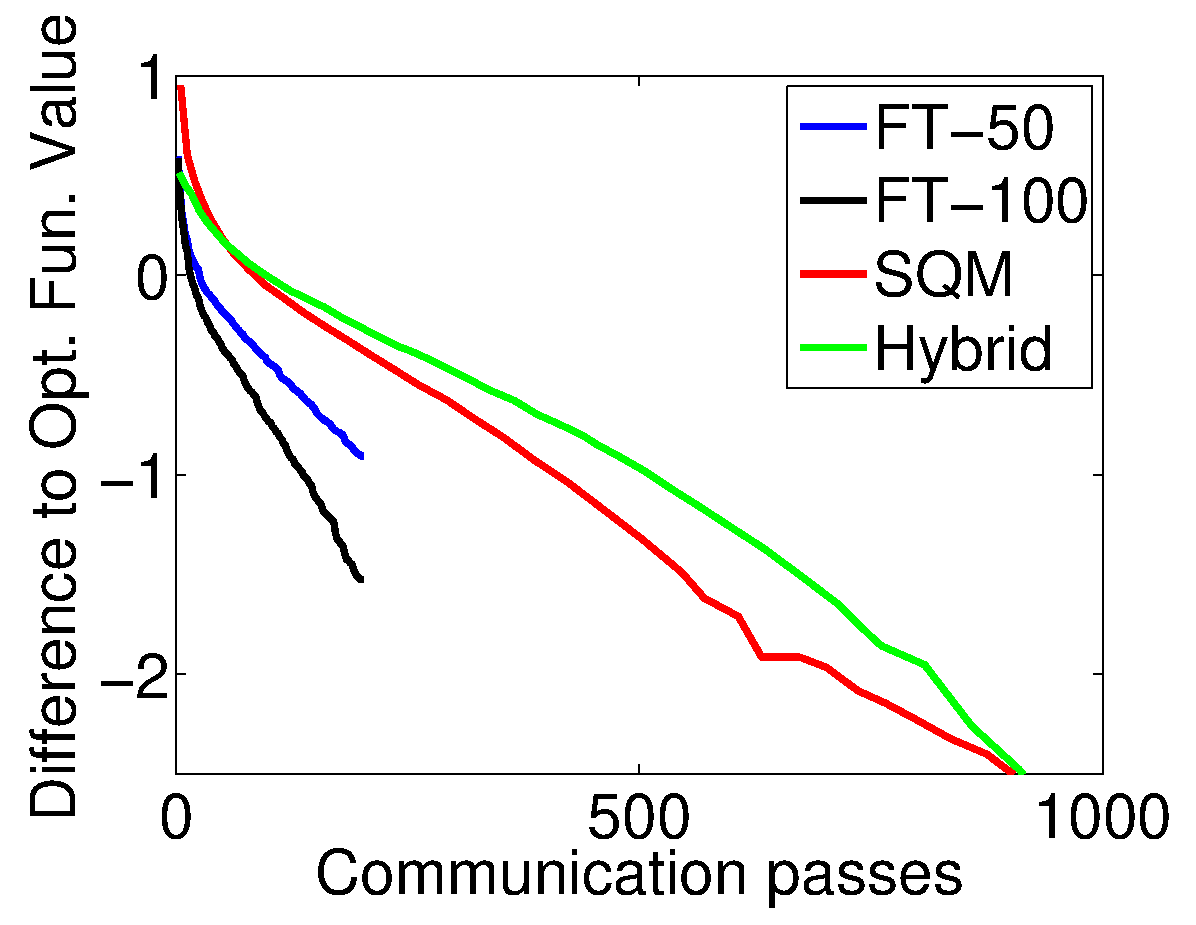
\includegraphics[width=0.46\linewidth]{figures/urltron_100nodes_outeriters.eps}
}
\label{commpass}
\caption{Plots showing linear convergence of our method using TRON as the local optimizer. $x$-axis is the number of communication passes and $y$-axis is the relative
decrease in function value in $\log_{10}$ scale.}
\end{figure}

\subsection{Results}
{\bf{Linear Convergence. }}To validate linear convergence,  we study the variation of $(f-f^*)/f^*$ (in log scale) as a function of the number of communication passes\footnote{Note that we do not use the number of outer iterations as x-axis because it has different meaning for different methods. For example for {\it{SQM}} and {\it{HYBRID}} each outer iteration requires different number of passes (Hessian-vector computations) over data and hence different communication also. However, our class of methods requires fixed number of passes over data as well as only 2 communication passes per outer iteration.}, where $f^*$ is the optimal function value. (We obtained $f^*$ by running the algorithm to get a very accurate solution.) For our algorithms ({\it{FS-k}} and {\it{FT-k }}), the number of communication passes is just twice the number of outer iterations. From Figure 1, we make the following observations for {\it{FT-k }} on the {\it{kdd2010}} dataset: (a) the rate of convergence is linear for both $P=25$ and $100$, (b) it is steeper when $P=25$. This steeper behavior for $P=25$ is expected because the functional approximation in each node becomes better as the number of nodes decreases. Note that, almost always, the rate of convergence is better in the early stages of the optimization and becomes steady in the end stages. We observed similar linear convergence behavior for {\it{FS-k}} also. Note that the slope is dependent on $k$ and remains nearly same when $k$ is sufficiently large and the number of examples per node is small (see for example, the {\it{kdd2010}} dataset when $P=100$). Similar observations hold for the URL dataset as well. Overall, this experiment clearly demonstrates: (a) the flexibility of our distributed algorithm in using any linear convergent local optimization algorithm, (b) a linearly convergent IPM algorithm and (c) a parallel SGD method (with its variants such as SVRG).

%shows the results of number of communication passes versus the difference to the optimal function value for different number of nodes ($P=6,25,100$.  Note that both {\it{FS-k}} and {\it{FT-k }} show overall linear convergence (straight lines) for different values of $k$. As expected, the rate of convergence (slope) increases (with diminishing returns) as we increase $k$ since the local optimization becomes more accurate. It also increases with decreasing number of nodes $P$ as the functional approximation becomes better.

{\bf{Time Taken. }}Figure 2 shows the timing results. We observe that there is an optimum value of $k$ for which we get the best result. This is because although the rate of convergence becomes better with increasing $k$ (as discussed above), the computation cost starts increasing and becomes dominant after a certain value of $k$. Moreover, the optimal $k$ value also decreases with increasing $P$. This happens because of two reasons. First, the computation cost increases with decreasing number of nodes. As a result the number of inner iterations that we can perform before the computation cost starts dominating the communication cost, decreases. Second, since the functional approximation becomes better as $P$ decreases, we require lesser number of iterations to get a good descent direction. As a result, our approach does well even if $k$ is small. From our experiments, we also observed that at the optimal $k$, neither communication cost nor computation cost dominates other completely. Hence, as a rule of thumb, the value of $k$ should be chosen (or selected in a range) such that both the costs balance each other.
%{\bf{TRON vs. SVRG:}} TO be completed once results are there

%{\bf{Other Methods: }}Figures~\ref{},~\ref{}and~\ref{} compare our method with {\it{HYBRID}} and {\it{SQM}}. For {\it{FS-k}} we used $k=$ while for {\it{FT-k }} $k$ was set to.

\begin{figure}[t]
\centering
\subfigure[25 nodes]{
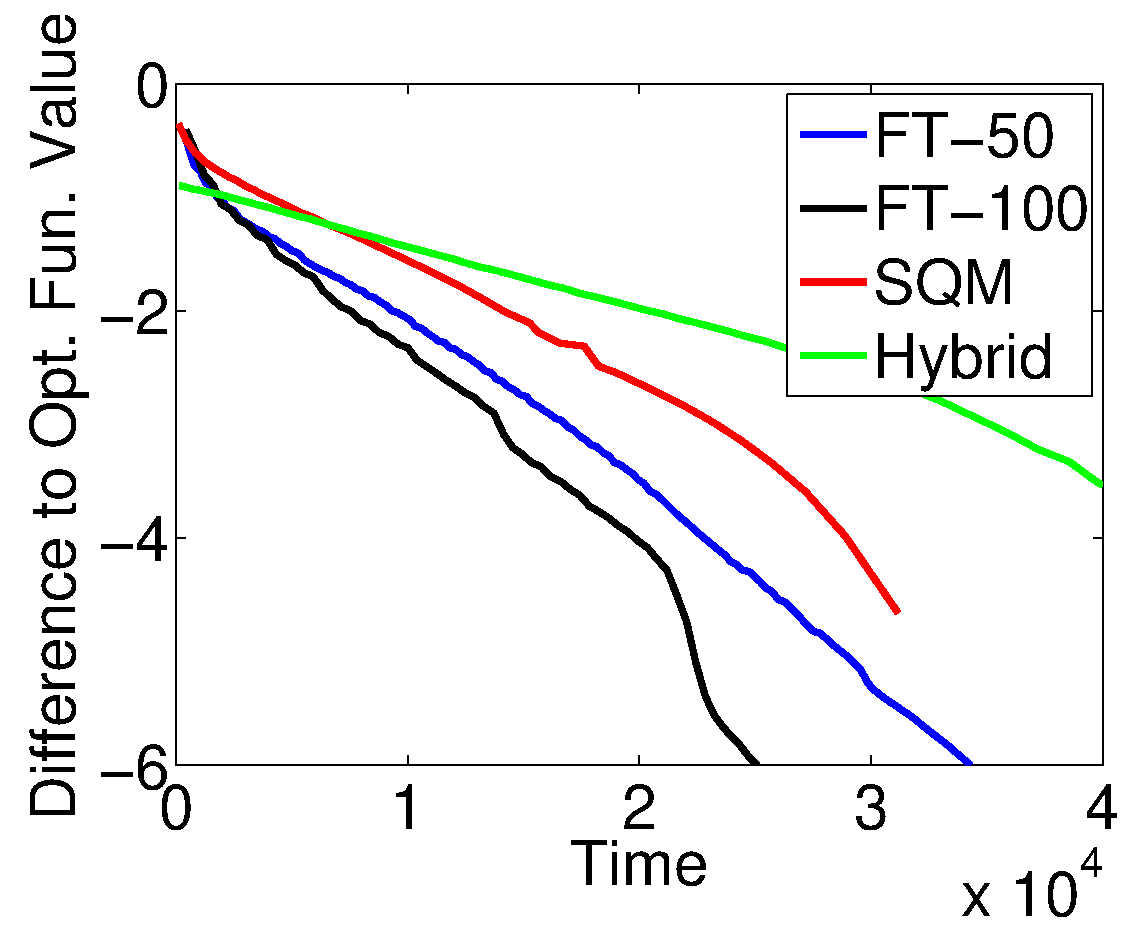
\includegraphics[width=0.46\linewidth]{figures/kddtron_25nodes_time.eps}
}
\subfigure[100 nodes]{
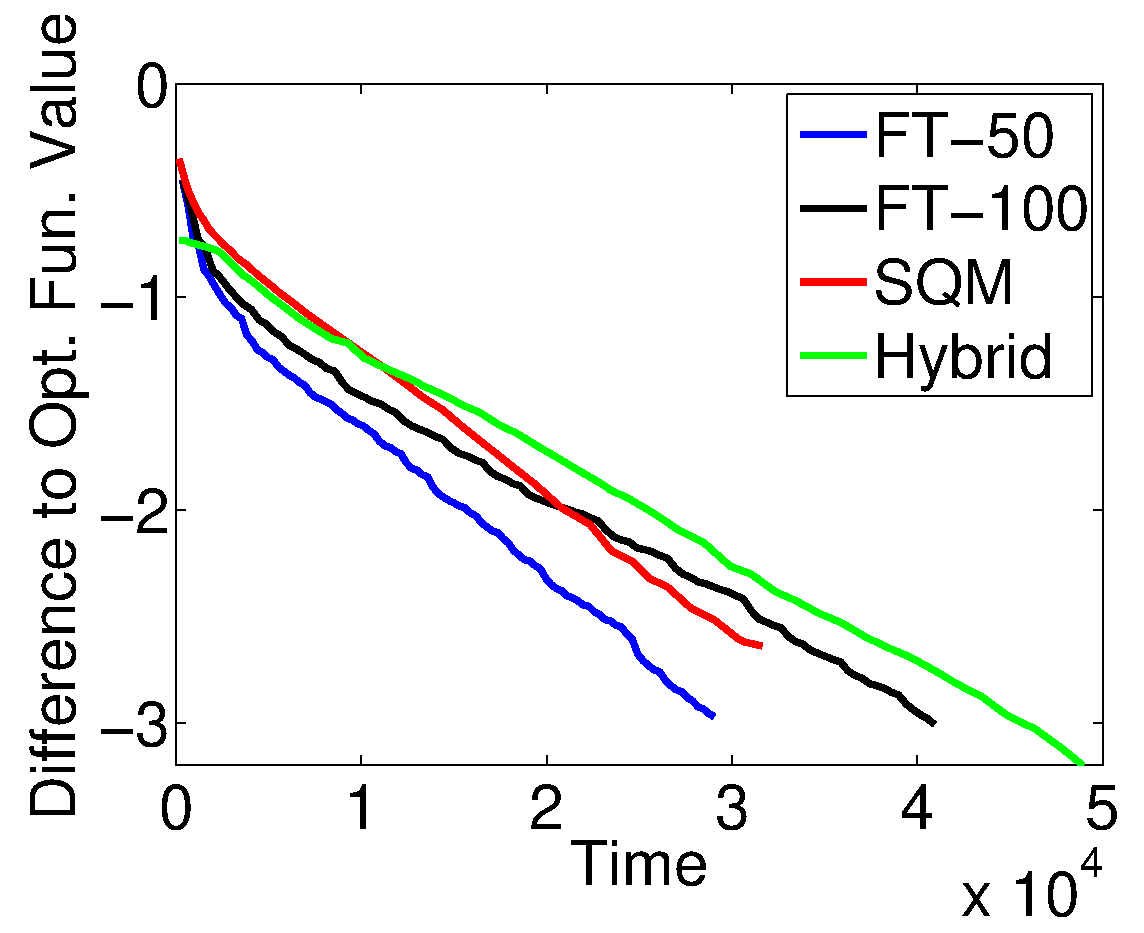
\includegraphics[width=0.46\linewidth]{figures/kddtron_100nodes_time.eps}
}
\subfigure[25 nodes]{
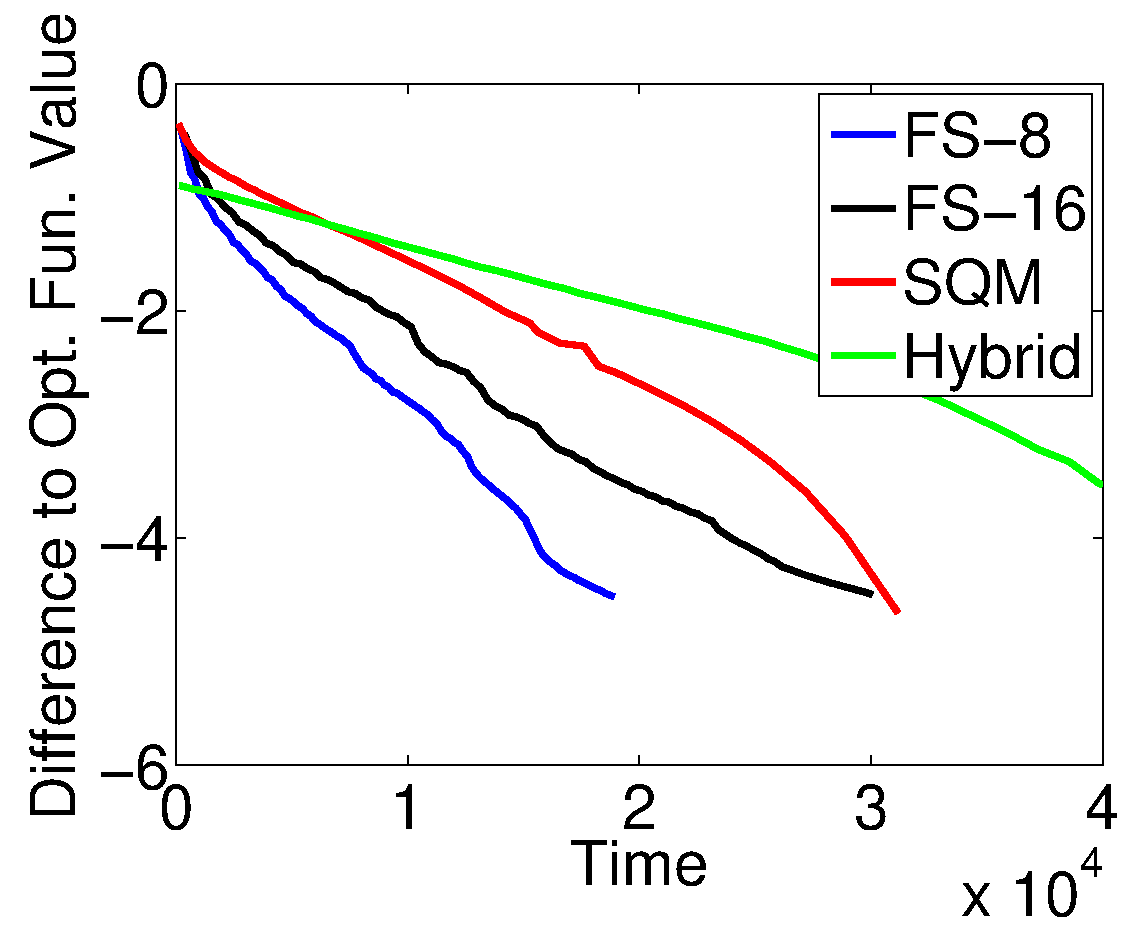
\includegraphics[width=0.46\linewidth]{figures/kddsvrg_25nodes_time.eps}
}
\subfigure[100 nodes]{
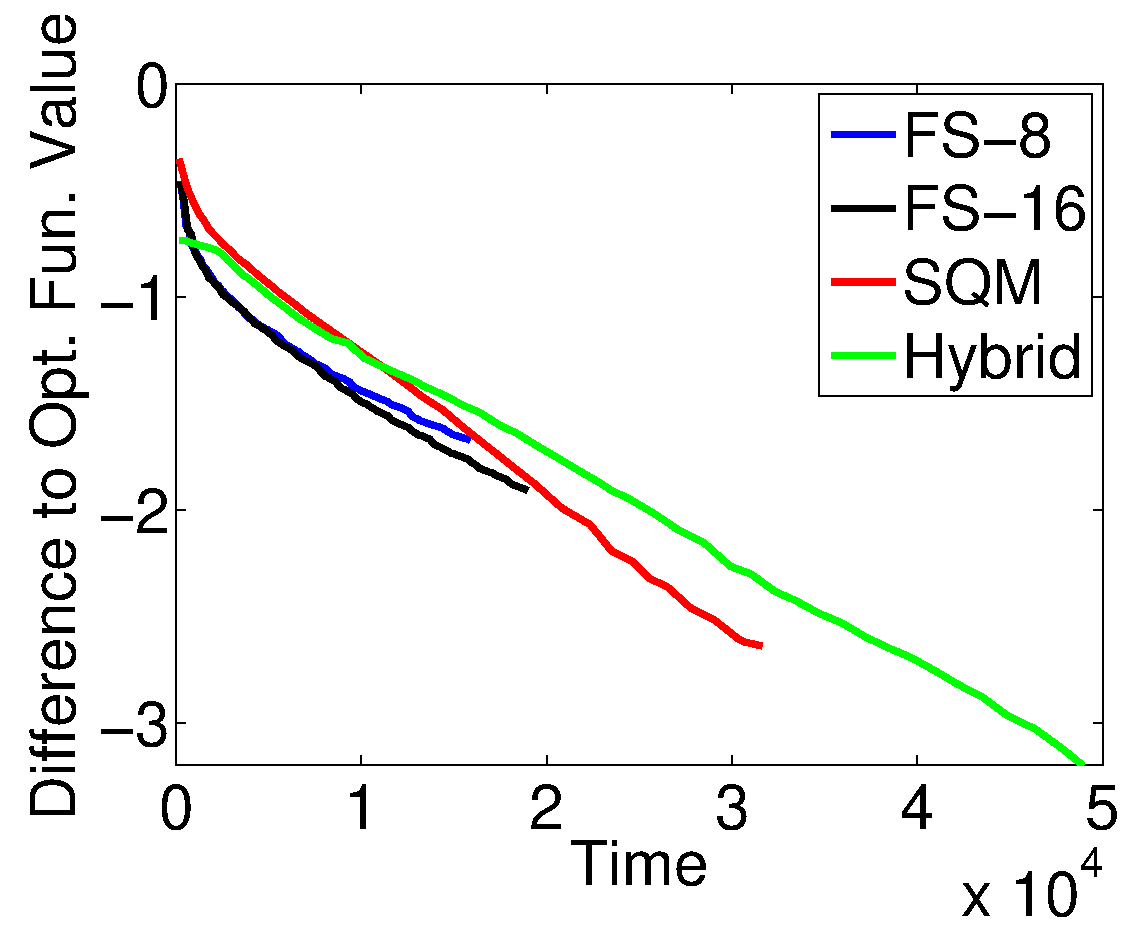
\includegraphics[width=0.46\linewidth]{figures/kddsvrg_100nodes_time.eps}
}
\caption{Plots showing overall linear convergence of our method and comparisons with {\it{SQM}} and {\it{HYBRID}} for {\it{kdd2010}}. $x$-axis is time (in seconds). Results are shown using with TRON and SVRG for local optimization.}
\label{timepass}
\end{figure}

{\bf Comparison with other methods. }For {\it{HYBRID}} and {\it{SQM}} algorithms, the number of communication passes is equal to the number of Hessian-vector and gradient computations. From Figures 1 and 2, we first see that {\it{HYBRID}} performs better than {\it{SQM}} due to warm start when the number of iterations are small. However, the performance difference between {\it{HYBRID}} and {\it{SQM}} decreases with increasing iterations and eventually {\it{SQM}} performs better. This behavior is a bit surprising and needs to be investigated.

\comment{
{\bf Comparison with other methods. }For {\it{HYBRID}} and {\it{SQM}} algorithms, the number of communication passes is equal to the number of Hessian-vector and gradient computations. From Figures 1 and 2, we first see that {\it{HYBRID}} performs better than {\it{SQM}} due to warm start when the number of nodes is small. This is expected because we expect the local model weight vectors to be closer to the global one (as more data is available in each node). The performance difference between {\it{HYBRID}} and {\it{SQM}} decreases with increasing number of nodes as the variance among the local models increases. In fact, for {\it{kdd2010}}, {\it{HYBRID}} performed worse than {\it{SQM}} for $P=100$.
}
Second, both {\it{FS-k}} and {\it{FT-k }} need significantly less communication passes ($3-5$ times) than {\it{HYBRID}} to reach moderately small relative error (say $10^{-3}$). In this case, our algorithms perform better in terms of time also. Note that as seen in Figure 3, this is sufficient to get a good AUPRC performance; also, our algorithms (both {\it{FT-k }} and {\it{FS-k}}) reach the stable performance much quicker than other algorithms. This clearly illustrates the usefulness of our distributed algorithm when communication cost is the bottleneck.

One other important point to note is: {\it{HYBRID}} and {\it{SQM}} start performing better when a very small relative error (e.g., $10^{-6}$) is desirable. This behavior can be explained as follows: In the beginning of the optimization, our functional approximation gives a good global view to all the nodes. As a result, we perform better than {\it{SQM}} and {\it{HYBRID}} by doing multiple inner iterations on this global approximation. However, closer to the optimum, the function curvature starts dominating the rate of convergence. Since {\it{SQM}} and {\it{HYBRID}} have better curvature estimates (available via global Hessian) they start performing better near the optimal solution. Hence, in summary, our approach has good global convergence but slow local movement (i.e., near the optimal solution) while {\it{SQM}} and {\it{HYBRID}} have slow global convergence but good local movement. Although theoretically one can incorporate second order functional approximation in our approach also, effectively communicating the Hessian information can be challenging. In future, we would like to incorporate ideas from Quasi-newton algorithms like L-BFGS~\cite{liu89} in our functional approximation and develop hybrid algorithms that switch to {\it{SQM}} at some point in our method.

%We also notice that the gap between our methods and {\it{SQM}} and {\it{HYBRID}} decreases with increasing number of nodes. This happens because our functional approximation becomes cruder as $P$ increases. The exact $P$ up to which our approach performs better varies from dataset to dataset and depends on the learning curve. For steeper learning curves, our performance should degrade slower. The exact analysis is left as a future work. Similar observations can be made on the time curves in Figure~\ref{}.

%Finally, Figure~\ref{} shows time versus AUPRC results for different methods. Our method clearly outperforms both {\it{HYBRID}} and {\it{SQM}} in getting good AUPRC values (within $0.5\%$ of the optimal).

To conclude, our functional approximation based distributed learning algorithm is flexible and fills several gaps in the literature. We have demonstrated that our algorithms work well when (a) the number of features is very large, (b) the functional approximation is good, and (c) moderately small relative objective function error is desired. We expect to come up with better functional approximations and hybrid algorithms in the near future that does well under all conditions.





\begin{figure}
\centering
\subfigure[25 nodes]{
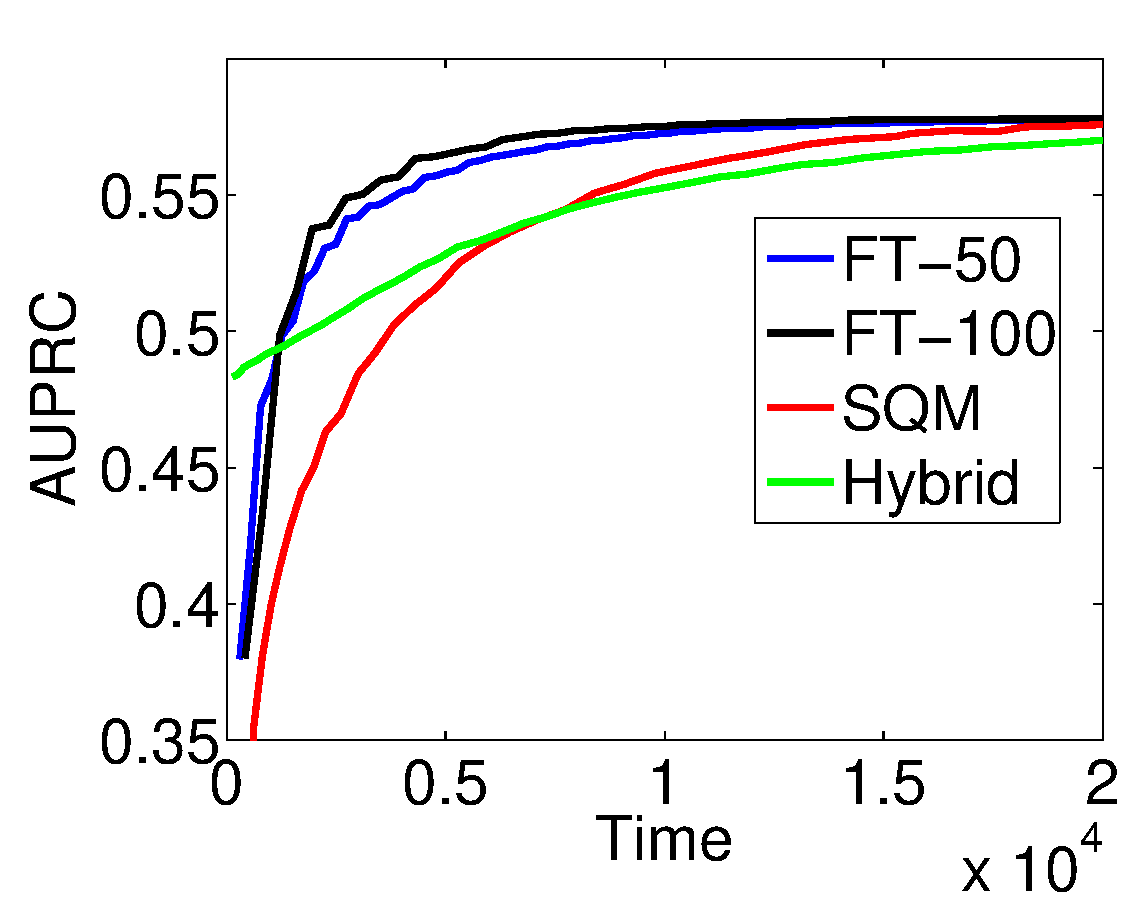
\includegraphics[width=0.46\linewidth]{figures/kddtron_25nodes_auprc.eps}
}
\subfigure[100 nodes]{
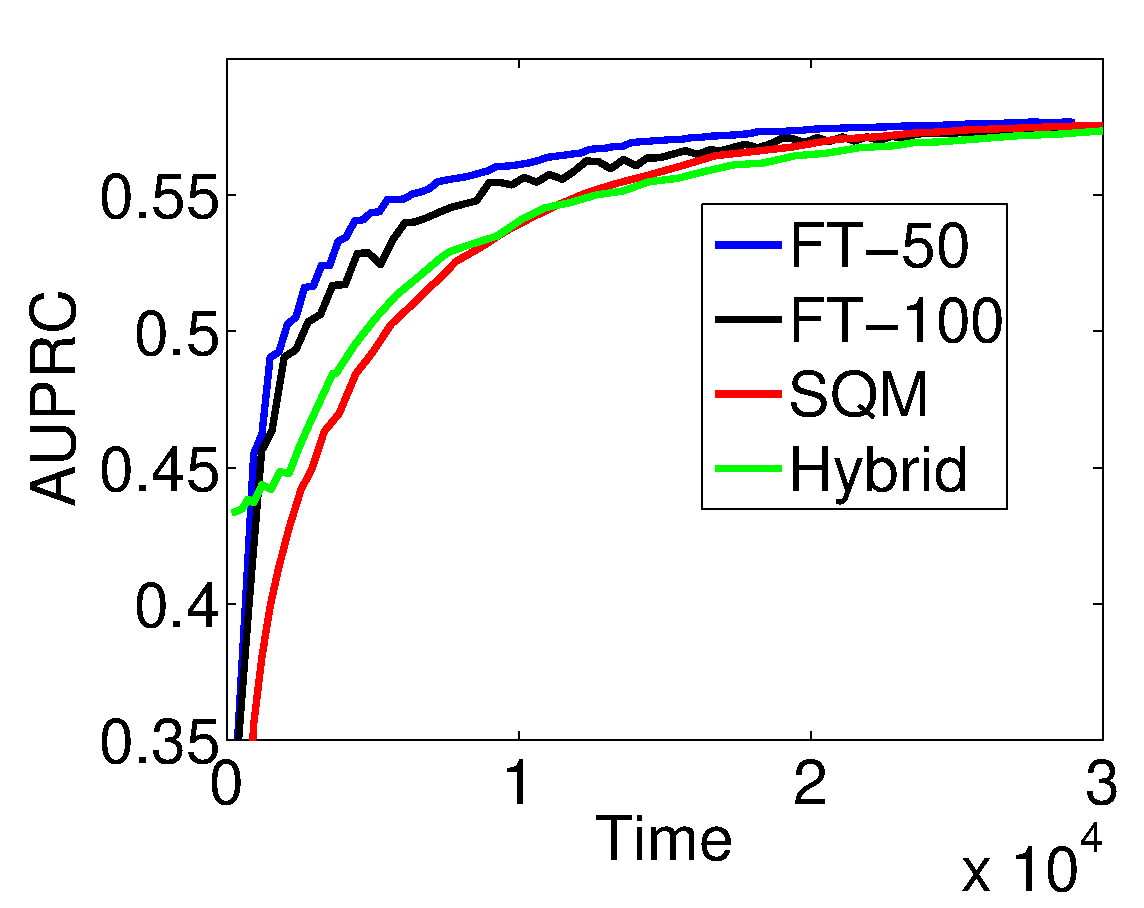
\includegraphics[width=0.46\linewidth]{figures/kddtron_100nodes_auprc.eps}
}
\subfigure[25 nodes]{
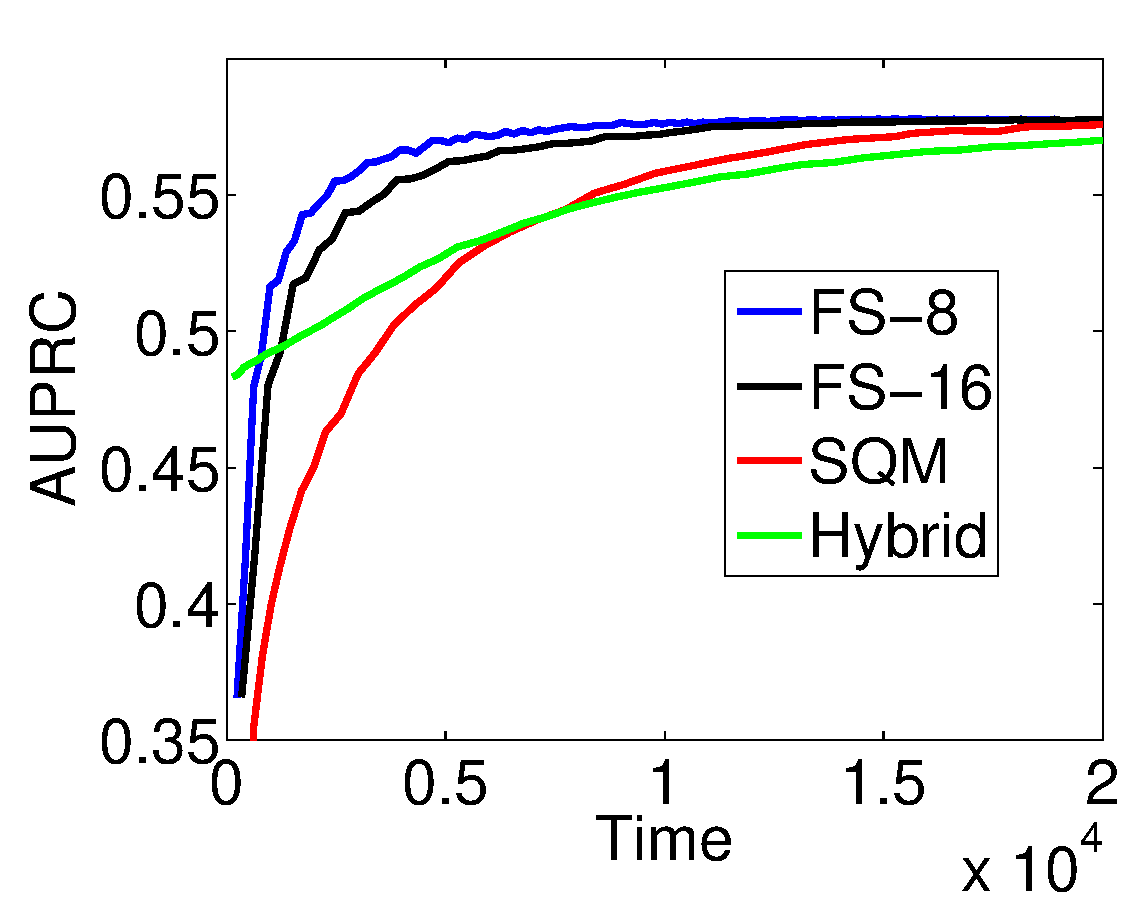
\includegraphics[width=0.46\linewidth]{figures/kddsvrg_25nodes_auprc.eps}
}
\subfigure[100 nodes]{
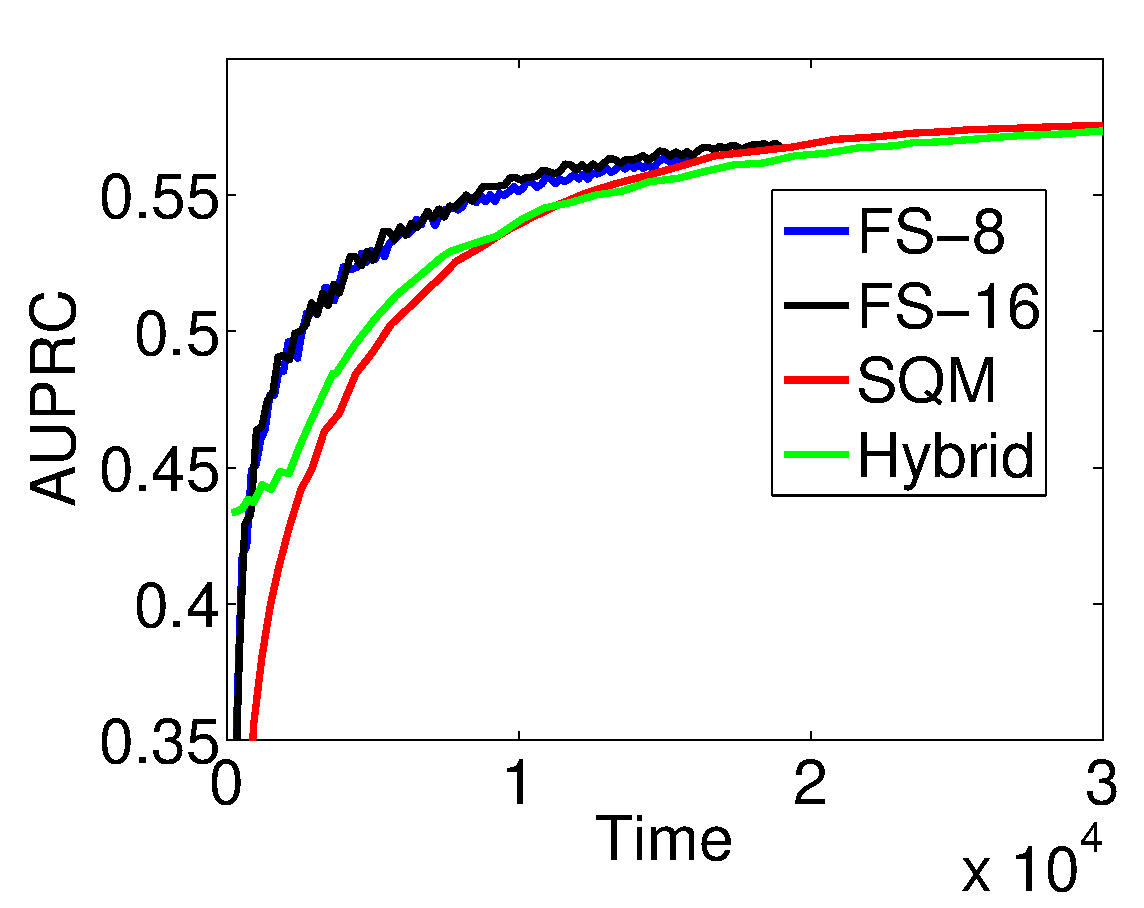
\includegraphics[width=0.46\linewidth]{figures/kddsvrg_100nodes_auprc.eps}
}
\caption{Plots showing AUPRC metric for our method, {\it{SQM}} and {\it{HYBRID}} for {\it{kdd2010}}. $x$-axis is time (in seconds).}
\label{auprc}
\end{figure}

